\section{Chain operations and evolution: main-chain pruning, collateral maturity, and post-quantum migration}
\label{sec:chain-evolution}\label{sec:chain-ops}

The roadmap groups three chain-level changes under a single H1 2027 heading, and a reader could be
forgiven for assuming they are equally ready because they share a quarter
\srcroadmap{H1 2027 chain-changes section}. They are not. One of them, main-chain pruning, is
already-shipped software wired into \fluxd; the operational decision is what is new. The second,
collateral maturity, is a named consensus-rule proposal with an explicit open item that decides
whether it works at all. The third, post-quantum migration, has a deliverable for H1 2027 that is a
published plan, not a change to any key. This section keeps the three separate, states a maturity
tag and a feasibility class for each, and closes with the constraint all three share: none of them can
rotate a key the protocol does not itself control. Collateral maturity delays when an existing key may
spend; it does not replace that key. Post-quantum migration is precisely the case in which the
protocol would like to replace a key and structurally cannot without the key-holder's cooperation.

\begin{figure}[H]
\centering
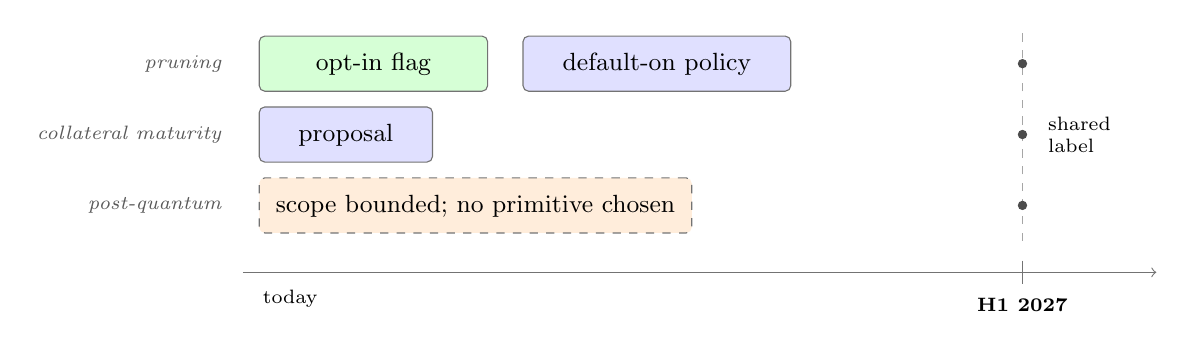
\begin{tikzpicture}[font=\small,
  track/.style={rounded corners=2pt, minimum height=7mm, text height=1.6ex, text depth=.4ex,
                draw=black!55, inner xsep=6pt},
  ship/.style={track, fill=green!16},
  plan/.style={track, fill=blue!12},
  vis/.style={track, fill=orange!14, dashed},
  lbl/.style={font=\scriptsize\itshape, text=black!65},
]
% shared time axis
\draw[->, black!55] (0,-0.1) -- (11.6,-0.1);
\node[font=\scriptsize, anchor=north] at (0.6,-0.2) {today};
\draw[black!55] (9.9,0.05) -- (9.9,-0.25);
\node[font=\scriptsize\bfseries, anchor=north] at (9.9,-0.3) {H1 2027};

% pruning
\node[lbl, anchor=east] at (-0.15,2.55) {pruning};
\node[ship, anchor=west, minimum width=2.9cm] at (0.2,2.55) {opt-in flag \shipped};
\node[plan, anchor=west, minimum width=3.4cm] at (3.55,2.55) {default-on policy \planned};

% collateral maturity
\node[lbl, anchor=east] at (-0.15,1.65) {collateral maturity};
\node[plan, anchor=west, minimum width=2.2cm] at (0.2,1.65) {proposal \planned};

% post-quantum
\node[lbl, anchor=east] at (-0.15,0.75) {post-quantum};
\node[vis, anchor=west, minimum width=5.4cm] at (0.2,0.75) {scope bounded; no primitive chosen \vision};

% the shared marker
\draw[black!35, dashed] (9.9,0.3) -- (9.9,3.0);
\foreach \y in {2.55,1.65,0.75} \fill[black!70] (9.9,\y) circle (1.7pt);

\node[anchor=west, font=\scriptsize, text width=1.5cm, align=left] at (10.1,1.65)
  {shared \\ label};
\end{tikzpicture}
\caption{Three chain-evolution tracks that the roadmap places under one ``H1 2027'' label, shaded by
\emph{maturity} rather than by calendar position. The label is shared; the readiness is not. Pruning
exists as an opt-in flag today and needs a policy decision to become a default; collateral maturity is
a proposal with no code path in \fluxd yet; post-quantum migration has a bounded scope and no chosen primitive, and is the only
one of the three whose hardest sub-problem (\Cref{rem:pq-disposition}) is unsolved industry-wide. A
reader who takes the shared date as shared readiness would mis-plan all three.}
\label{fig:chain-evolution-tracks}
\end{figure}

\subsection{Main-chain pruning: an operational decision, not a new capability}

\texttt{-prune} is standard, inherited Bitcoin/Zcash functionality and is fully wired in \fluxd today
\shipped\ \srccode{fluxd/\allowbreak{}src/\allowbreak{}init.cpp}{986--1064, 1919} \srccode{fluxd/\allowbreak{}src/\allowbreak{}main.cpp}{4312--4313, 5930}.
\texttt{n\allowbreak{}Prune\allowbreak{}After\allowbreak{}Height} is set to $100{,}000$ on mainnet \srccode{fluxd/\allowbreak{}src/\allowbreak{}chainparams.cpp}{181}. No
\PoN-specific pruning constraint was found in the code. So ``main-chain pruning'' as a roadmap item is
not the implementation of a new capability; it is the decision to turn on a capability that already
exists, together with the archival tier that has to sit beside it once history is no longer kept by
every node \srcroadmap{Main-chain pruning, H1 2027}.

The roadmap's own justification is that pruned nodes remain able to produce blocks:

\begin{quote}
``30-second blocks mean the chain grows quickly. Pruning cuts what a node must store and speeds up
syncing. Done properly, pruned nodes stay fully able to produce blocks, with designated archive nodes
preserving full history for explorers and the data services above.''
\srcdoc{flux-roadmap-public.md:121-122}
\end{quote}

Under \PoN\ this is a claim worth proving rather than restating, because block production requires two
things that a naive reading of ``pruning'' might endanger: evaluating slot eligibility
$H(\text{collateral} \Vert \text{prevHash} \Vert \tslot) \le \text{target}$ and signing
\srccode{fluxd/\allowbreak{}src/\allowbreak{}pon/\allowbreak{}pon.cpp}{70--86}, and validating the \FluxNode\ registry against which that
collateral outpoint is checked. The reason the claim holds is that the registry does not live inside
the block store it would otherwise be pruned along with: \FluxNode\ state is a single global structure,
\texttt{g\_fluxnode\allowbreak{}Cache}, persisted in its own LevelDB database keyed by datadir path
\texttt{determ\_zelnodes} \srccode{fluxd/\allowbreak{}src/\allowbreak{}fluxnode/\allowbreak{}fluxnodecachedb.cpp}{26}, and is rebuilt from that
store at every startup independently of how much of the block chain is retained
\srccode{fluxd/\allowbreak{}src/\allowbreak{}fluxnode/\allowbreak{}fluxnodecachedb.cpp}{49--79}.

\begin{property}
A pruned \PoN\ node retains block-production capability if and only if the \FluxNode\ registry and the
UTXO set for collateral outpoints are retained, regardless of pruning depth.
\end{property}

This is stateable precisely because the registry already lives outside the block store rather than
being derived from block history on demand; a chain whose node registry had to be replayed from full
block history would not have this property, and \fluxd's separation of the two stores is what makes
pruning and \PoN\ compatible without further engineering \shipped\
\srccode{fluxd/\allowbreak{}src/\allowbreak{}fluxnode/\allowbreak{}fluxnodecachedb.cpp}{26,49--79}.

\begin{remark}[Archival is a tenant product, not a node obligation --- settled]
\label{rem:archive-product}
The pruning-depth policy and the archival-redundancy target were carried as open. They are settled by
a decision that resolves both at once and relocates the problem: \textbf{archive nodes are
applications running on \FluxCloud}. The team deploys them as tenant workloads and sells access to
RPC and other node APIs as a product \srcintent{08-answers-round-2.md, round 16} (\planned).

Two consequences, and the second is the one worth stating carefully.

\emph{Pruning is unconstrained by any retention obligation.} If no node is obliged to keep history,
the pruning-depth policy is a storage-efficiency choice for ordinary operators rather than a
network-safety parameter, and it can be set as aggressively as operators want. The awkward coupling
that made this an open question --- how deep can we prune without endangering history --- dissolves,
because history is not being kept by the pruning nodes in the first place.

\emph{History availability becomes a function of demand for a product.} This is the honest form of
the trade and the paper states it plainly: if archival capacity is a paid service, then history
survives exactly as long as someone finds it worth paying for. That is a different guarantee from
``every node keeps everything'', and it is weaker in a specific way --- there is no protocol rule
setting a minimum number of archive nodes, so the redundancy target is a commercial decision, not a
consensus one. A chain whose full history rests on the commercial viability of an archive product
should say so, and this one does.
\notestablished{no redundancy target for archive deployments is stated in any artefact read
for this paper, and none is derivable from the decision that archival is a product. The number of
independent archive deployments required before history is durable is therefore not stated here.}
\end{remark}

The roadmap pairs pruning with a paid product built from the archive nodes pruning requires, describing
RPC, archive and indexing services as the network's ``first capacity-selling product'' and stating that
this ``pairs directly with chain pruning: the archive nodes pruning requires become the product''
\srcdoc{flux-roadmap-public.md:33-34}. This is the clearest instance in the deployed system of the
demand-funded thesis applied to the chain layer itself: an operational cost the network would otherwise
carry for free (full history) becomes a service the network sells, and the archive tier pruning makes
necessary is the same tier that generates the revenue. \srcroadmap{RPC, archive and indexing services,
Q3 2026}

See \Cref{rem:archive-product}: archival capacity \emph{is} a paid product, deployed as
\FluxCloud{} applications, and the consequence for history availability is stated there rather than
left conditional. \srcinferred

\textbf{Class: Extension.} The mechanism exists; what remains is the operational decision to enable it
and the archival-capacity policy above.

\subsection{Collateral maturity: a proposal, not yet a rule}

Collateral maturity is not deployed and has no code path in \fluxd today; the roadmap presents it
explicitly as a proposal that has not yet gone to operators \srcroadmap{Collateral maturity, H1 2027}
\planned. The stated rule is a rolling maturity on the collateral outpoint, modelled on coinbase
maturity:

\begin{quote}
``For attestation to carry real weight, a node's stake in the network has to outlast the window in
which its claims can be challenged. We will propose a consensus rule: a node-collateral UTXO becomes
spendable only 30 days after the node's last confirmed activity — a rolling maturity, like coinbase
maturity, applied prospectively and never to standing collateral. Moving collateral directly into a new
or upgraded node (including into multisig custody) stays instant; only leaving waits. There is no
confiscation and never will be.'' \srcdoc{flux-roadmap-public.md:143-144}
\end{quote}

Formally: for a collateral outpoint $o$ with last confirmed activity height $\hgt_{\mathrm{act}}(o)$,
spending $o$ would be valid at height $\hgt$ if and only if
\[
\hgt \;\ge\; \hgt_{\mathrm{act}}(o) + M
\qquad\text{or}\qquad
\mathrm{dest}(o) \in \mathcal{D}_{\text{node}},
\]
with $M = 86{,}400$ blocks — 30 days at the \PoN\ target spacing $\spacingpon = 30\,\mathrm{s}$ — and
$\mathcal{D}_{\text{node}}$ the set of destinations that constitute continued participation.

\notestablished{the definition of $\mathcal{D}_{\text{node}}$ --- which destinations count as
continued participation, so that a move into a new or upgraded node or into multisig custody stays
instant while an exit disguised as a move does not --- is stated in no artefact read for this paper.
It is the parameter on which the rule's acceptability rests: too permissive and the rule does
nothing, too restrictive and funds are held by a mechanism promised not to hold them.}

\proposednote{$M = \num{86400}$ blocks is this paper's recommendation, and the constraint that made
it non-free-standing is satisfiable: it must satisfy $M \ge \Delta_{\mathrm{chal}}$, and
\S\ref{sec:attested-execution} recommends $\Delta_{\mathrm{chal}} = \num{2880}$ blocks. With
$\num{86400} \ge \num{2880}$ the constraint holds with a factor of \num{30} in hand, so $M$ can be
treated as a free choice after all --- and it reuses the \PNR{} constant $K$, so one number serves
three mechanisms. \srcinferred.}

Non-retroactivity is stated as part of the proposal and is what makes it non-confiscatory:

\begin{property}
For every collateral outpoint existing before the activation height $\hgt_{\mathrm{act}}^{\star}$, the
maturity rule does not apply: no standing collateral is retroactively locked.
\end{property}

The roadmap also states a second-order effect openly rather than leaving it to be found later — a
maturity rule smooths collateral unlock waves — and frames this as a proposal that would ride an
already-planned network upgrade rather than force its own:

\begin{quote}
``We state the second-order effect ourselves rather than leaving it to be discovered: a maturity rule
also smooths collateral unlock waves. Both effects are the point. This is a proposal — it goes to
operators for discussion before any activation is scheduled, and it would ride an already-planned
network upgrade rather than forcing its own.'' \srcdoc{flux-roadmap-public.md:146}
\end{quote}

Stated honestly, the rule buys a bounded window rather than permanence: an operator willing to stop
operating and wait $M$ blocks can still exit with the collateral intact, exactly as before the rule
existed. What the maturity rule changes is the cost of lying about continued participation while
attempting to exit early; what makes lying about an attestation claim actually costly is the bond
described in Section~14, not the maturity window itself. Section~8 and Section~14 divide the labour
this way: the maturity window guarantees stake outlasts a challenge; the bond is what is at risk if the
challenge succeeds.

\textbf{Class: Engineering.} There is no unsolved technical problem in the maturity rule as stated; the
open item is the definition of $\mathcal{D}_{\text{node}}$, and the real cost is the political work of
operator consent the roadmap itself names as a prerequisite \srcroadmap{Collateral maturity, H1 2027}.

\subsection{Post-quantum migration: a scope decision and an open problem}

The H1 2027 deliverable is a published migration path, not a migration:

\begin{quote}
``The realistic threat is store-now-decrypt-later, not live breakage. We publish a migration path on
the NIST-standardised signature schemes. Migration itself is a multi-year effort — this is where
Bitcoin and Ethereum are too.'' \srcdoc{flux-roadmap-public.md:148-149}
\end{quote}

\vision\ \srcroadmap{Post-quantum roadmap, H1 2027}. Consistent with that, a repository-wide grep for
the obvious primitive names returns nothing: \srccode{fluxd/\allowbreak{}src}{repo-wide grep for
\texttt{quantum|dilithium|kyber|falcon|sphincs|schnorr}: zero hits outside a vendored
\texttt{secp256k1/\allowbreak{}.\allowbreak{}gitignore}}. No post-quantum code, comment, or dependency exists in \fluxd\ today.

\paragraph{What is at risk.} The signature primitives at risk are all classical-ECDSA over
secp256k1: transparent-address spending; \FluxNode\ registration and confirmation signing, via
\texttt{Sign\allowbreak{}Deterministic\allowbreak{}Start\allowbreak{}Tx} and \texttt{Build\allowbreak{}Deterministic\allowbreak{}Confirm\allowbreak{}Tx}
\srccode{fluxd/\allowbreak{}src/\allowbreak{}fluxnode/\allowbreak{}activefluxnode.cpp}{253--288,380--407}; the \PoN\ block header's own
\texttt{vchBlockSig} field, an ECDSA signature over the block hash carried in every post-activation
header alongside the winning collateral outpoint \srccode{fluxd/\allowbreak{}src/\allowbreak{}primitives/\allowbreak{}block.h}{44--45,64--96};
the 2-of-4 emergency-block key set \srccode{fluxd/\allowbreak{}src/\allowbreak{}chainparams.cpp}{242--253}; and the
benchmark-signing key allowlist \srccode{fluxd/\allowbreak{}src/\allowbreak{}chainparams.cpp}{233--240}, alongside the
attestation-signing keys discussed in Section~14. Hashing is a separate matter: SHA-256 and the
historical chain's Equihash instantiation degrade only quadratically under a quantum adversary, which
is a general property of quantum search against hash-based primitives rather than a Flux-specific
finding, and is not the part of the system this scope decision needs to address \srcinferred.

\paragraph{The scope decision.} The team has settled, as design intent, that the post-quantum scope is
deliberately bounded to consensus, transparent transactions, and the keys securing them, with the
shielded layer explicitly excluded and deferred as the field matures, on the grounds that privacy is
optional on \Flux\ and the transparent layer is the one every user and every consensus rule depends on
\srcintent{05-privacy-pq.md} \vision. This is presented as a considered position, not a gap, and it
carries a consequence the paper states plainly because a reviewer would otherwise find it: Groth16, the
proving system underlying the shielded pool described in Section~20, rests on a pairing assumption and
is not post-quantum secure. An unqualified ``quantum-ready \Flux'' claim made alongside a live shielded
pool built on Groth16 would therefore be an error; the bounded scope stated here is exactly what avoids
making it \srcintent{05-privacy-pq.md}.

\textbf{The retirement decision simplifies this considerably.} With both shielded pools retired
(\S\ref{sec:shielded-retirement}), Groth16 leaves the consensus path altogether, and with it the one
component whose presence made a ``quantum-ready \Flux'' claim require careful qualification. After
retirement the post-quantum scope is not \emph{bounded} to transparent transactions --- it is
\emph{coextensive} with the chain, because transparent transactions and the keys securing them are
all that remains. That is a genuine simplification of the migration problem stated in this section,
and it was not among the reasons given for the decision, which makes it worth recording as a
consequence rather than a justification.

A related and separate point, kept separate deliberately: adopting Halo2/Orchard-class proving would
remove the shielded layer's inherited trusted setup, which is a real, independently motivated
improvement discussed in Section~20 --- but it would not make the shielded pool post-quantum secure,
since Halo2 rests on discrete-log hardness rather than a quantum-hard assumption. Eliminating a trusted
setup and achieving post-quantum security are different properties, and this section, Section~14, and
Section~20 must not conflate them \srcintent{05-privacy-pq.md}.

\paragraph{The migration problem.} Signature migration on a UTXO chain is not an ordinary protocol
upgrade, because the protocol cannot move funds it does not hold the key to.

\begin{openproblem}
Let $U_{\mathrm{cls}}$ be the set of outputs spendable only by a classical signature. No consensus rule
can move an output in $U_{\mathrm{cls}}$ without the corresponding private key. A store-now-decrypt-later
adversary harvests public keys revealed at spend time and, once a capable quantum adversary exists,
spends any output in $U_{\mathrm{cls}}$ whose public key it has recorded. A migration must therefore
(i) offer a post-quantum output type, (ii) incentivize or compel movement of value into it, and
(iii) decide what happens to outputs in $U_{\mathrm{cls}}$ that never move.
\end{openproblem}

Item (iii) has no good answer anywhere in the industry today, and the honest statement is that \Flux\
is in the same position as Bitcoin and Ethereum, not ahead of them \srcdoc{flux-roadmap-public.md:149}.
The design space for the disposition of unmoved classical outputs has three known shapes, each with a
distinct trade-off:

\begin{enumerate}
\item \emph{A flag-day freeze.} After a fixed height, any output in $U_{\mathrm{cls}}$ whose owner has
not moved it becomes permanently unspendable. This forces the migration but is confiscatory by
construction for anyone who cannot act in time — lost keys, custodial delay, simple inattention — which
is exactly the property the collateral-maturity rule above was designed to avoid.
\item \emph{A permanent classical tail.} Nothing is ever frozen; the network accepts that any output in
$U_{\mathrm{cls}}$ whose public key becomes known remains at risk indefinitely once a capable adversary
exists. Nothing is confiscated, but the exposure never closes.
\item \emph{A hash-based commitment allowing a post-quantum proof of prior ownership.} An owner could
later prove, using a post-quantum-secure proof, that they controlled a given classical output before
some cutover, without needing a pre-committed post-quantum key at the time of the original output.
This is the least destructive of the three on its face, but so far as this section's sources establish,
no production-grade construction of this kind is deployed anywhere at the scale a base-layer chain
would require \srcinferred.
\end{enumerate}

\begin{remark}[\FluxNode{} collateral public keys are already public, by protocol design]
\label{rem:pq-collateral-exposed}
The three dispositions above are the general framing, and it is the framing Bitcoin and Ethereum
share. \Flux{} is not in the same position, and the difference is material enough that the
disposition question has to be answered per class rather than once.

On a Bitcoin-derived chain the structural mitigation for unmoved funds is that a P2PKH output commits
to $\mathsf{HASH160}(pk)$ rather than to $pk$: the public key is not on the chain until the output is
spent, so an adversary running Shor's algorithm has nothing to attack. That protection does not exist
for \FluxNode{} collateral. The \texttt{collateral\allowbreak{}Pubkey} field is serialised directly into the
\FluxNode{} START transaction and written to the chain at registration \shipped
\srccode{fluxd/src/primitives/transaction.h}{1038--1039};
\srccode{fluxd/src/fluxnode/activefluxnode.cpp}{368}. Every operating node has therefore
\emph{published} its collateral public key as a condition of operating, permanently and in the clear.

\begin{table}[H]
\centering\footnotesize
\caption{Collateral whose public keys are on-chain by protocol design. Node counts and tier split
\shipped \srcmeasured{\texttt{listzelnodes}}{2026-09-03}; supply from the emission model at height
\num{2912015}.}
\label{tab:pq-exposure}
\begin{tabular}{@{}lrrr@{}}
\toprule
Tier & Nodes & Collateral each (\flux) & Tier total (\flux) \\
\midrule
Cumulus & \num{3247} & \num{1000} & \num{3247000} \\
Nimbus & \num{1615} & \num{12500} & \num{20187500} \\
Stratus & \num{1627} & \num{40000} & \num{65080000} \\
\midrule
\textbf{Total} & \textbf{\num{6489}} & & \textbf{\num{88514500}} \\
\multicolumn{3}{@{}l}{Share of issued supply (\num{429466824}\flux)} & \textbf{\SI{20.61}{\percent}} \\
\bottomrule
\end{tabular}
\end{table}

\noindent \textbf{So roughly one fifth of issued supply sits in outputs that a cryptographically
relevant quantum computer could spend immediately}, without waiting for the owner to reveal anything,
and that fraction is not the result of user carelessness --- it is what the registration protocol
requires. This is a genuine architectural disadvantage relative to Bitcoin on this specific axis, and
the paper states it rather than inheriting Bitcoin's more comfortable framing.

\textbf{A correction this paper owes its own earlier reasoning.} An earlier draft concluded that
option (iii) --- a post-quantum proof of prior ownership --- was \emph{unavailable} for
\FluxNode{} collateral, on the argument that such a proof rests on the owner knowing a secret the
adversary cannot compute, which fails once $pk$ is published and Shor yields the private key. That
argument is wrong, and Bitcoin's own work shows why: the secret need not be the private key.
BIP-361 rests its rescue path on the knowledge asymmetry created by \textbf{BIP-32 hardened
derivation} \citep{bip361}. A hardened step derives the child key through a one-way function of the
parent seed, so recovering the child private key does not yield the seed. An owner can therefore
prove \emph{``I know a seed and a path that derive this key''} while a quantum adversary holding the
private key cannot. Option (iii) survives public-key exposure, provided the key was seed-derived
through a hardened step --- which is the normal case for wallet-generated keys and not the case for
raw imported ones.

So the design space for \FluxNode{} collateral does \emph{not} collapse to freeze-or-expose. It
collapses to something better, and \S\ref{sec:pq-frontier} builds on it.
\end{remark}

\subsection{The frontier: what Bitcoin is building, and the one move Flux can make that it cannot}
\label{sec:pq-frontier}

Bitcoin is the right comparison for this problem, because it faces the same one at larger scale and
its work is public, specified and adversarially reviewed. Two proposals define the current state of
that art, and \Flux{} should be read against them rather than against a generic notion of
``quantum readiness''.

\textbf{BIP-360} defines \emph{Pay-to-Merkle-Root} (P2MR): an output type offering nearly the
functionality of P2TR with the key-path spend removed, so that no internal public key is exposed and
a long-exposure attack by a cryptographically relevant quantum computer has nothing to work on. It is
Draft status, and it deliberately introduces \emph{no} post-quantum signature scheme --- the
algorithm choice is left to later work \citep{bip360}. \textbf{BIP-361} supplies the migration
policy: Phase~A, at \num{160000} blocks after activation, disallows sending funds \emph{to}
quantum-vulnerable addresses; Phase~B, two years later, tightens verification of ECDSA and Schnorr
signatures, freezing what has not moved. Its authors reject allowing theft outright, and its rescue
path rests on the hardened-derivation asymmetry described above --- with zk-STARK and commit-reveal
named as candidate proof systems and the honest admission that how much supply such a protocol could
cover ``remains to be seen'' \citep{bip361}. As of 2026-03-01, over \SI{34}{\percent} of all bitcoin
had revealed a public key on chain \srcinferred.

\paragraph{Where \Flux{} sits against that.} Two differences matter, and they point in opposite
directions.

\emph{Worse:} Bitcoin's exposed fraction is the product of user \emph{behaviour} --- spending, address
reuse --- and it grows monotonically because each spend reveals a key. \Flux's exposed fraction for
node collateral is the product of \emph{protocol mandate}: \SI{20.61}{\percent} of supply
(\Cref{tab:pq-exposure}) is exposed because the START transaction requires it, and an operator cannot
decline. No amount of careful user behaviour reduces it.

\emph{And a consequence Bitcoin's approach would not fix:} BIP-360's remedy is an output type that
hides the key in the \emph{scriptPubKey}. That does not help \Flux, because \Flux{}'s collateral
exposure is not in the output script at all --- it is in the \texttt{collateral\allowbreak{}Pubkey} field of the
\FluxNode{} transaction \srccode{fluxd/src/primitives/transaction.h}{1038--1039}. Adopting a
P2MR-equivalent output type would leave the exposure exactly where it is. \textbf{The registration
transaction format is what would have to change}, and that is a \Flux-specific problem with no
upstream solution to inherit.

\emph{Better, and decisively:} \textbf{\Flux{} has a mandatory, recurring, authenticated channel to
precisely the exposed set, and Bitcoin has none.} Bitcoin cannot reach a dormant holder; its only
instruments are to stop new exposure, to freeze, and to hope a rescue proof covers enough. Every
\Flux{} node, by contrast, must broadcast a START transaction to register and CONFIRM transactions to
keep being paid. The set with exposed keys \emph{is} the set transacting regularly and drawing income
--- and that turns an unreachable population into a reachable one.

\begin{remark}[Pre-staged commitment: the move the mandatory registration makes available]
\label{rem:pq-prestage}
The recommendation of \Cref{rem:pq-disposition} is eligibility-forced migration, and the team has
adopted it \srcintent{08-answers-round-2.md, round 15} (\planned). The frontier version of it exploits
a timing asymmetry that Bitcoin cannot use, and costs almost nothing to start now.

Extend the \FluxNode{} START and CONFIRM transactions with a \textbf{post-quantum key commitment}: a
pair $(\mathsf{alg\_id}, H(pk_{\mathrm{pq}}))$, the algorithm identifier and a hash of a
post-quantum public key the operator controls. Three properties make this the right shape.
\begin{enumerate}
  \item \textbf{It is nearly free to add, because the transaction is already mandatory.} These
  transactions already carry a public key and are already broadcast by every node on a schedule. A
  commitment field is marginal cost on a message that must be sent anyway --- which is exactly the
  cost structure Bitcoin does not have, because it has no mandatory message.
  \item \textbf{It commits to a hash, not a key, and names its algorithm.} Publishing
  $pk_{\mathrm{pq}}$ itself would recreate the long-exposure problem one algorithm later; publishing
  $H(pk_{\mathrm{pq}})$ does not. Carrying $\mathsf{alg\_id}$ keeps the scheme agile, so the NIST
  primitive can be chosen later without invalidating commitments made earlier --- and
  \S\ref{sec:pq-scope} is explicit that no primitive is chosen yet.
  \item \textbf{It inverts the migration.} If commitments are collected from today, then by the time
  a CRQC is credible every economically active node already has a post-quantum key committed on
  chain, and the cutover is a \emph{flag}, not a migration: consensus begins requiring a
  $pk_{\mathrm{pq}}$-authorised spend path, and the keys it needs are already there. Bitcoin's
  Phase~A/Phase~B schedule spends roughly five years doing what a mandatory registration channel can
  pre-stage silently.
\end{enumerate}

\textbf{And no collateral is ever frozen.} This is the substantive divergence from BIP-361, which
chooses freezing and defends the choice against the alternative of tolerated theft
\citep{bip361}. \Flux{} does not face that dilemma for its largest exposed class, because eligibility
does the work freezing does: a node that has not committed and migrated stops being confirmed and
stops earning, while its collateral stays spendable by its owner. The instrument is an income
incentive rather than a confiscation, and it applies continuously rather than at a flag day.

\paragraph{What this does not solve.} Two residues, stated rather than absorbed. Collateral held
behind \emph{raw imported} keys has no seed to prove derivation from, so the hardened-derivation
rescue does not reach it; those operators must migrate or lose eligibility, with no fallback. And
ordinary transparent outputs outside the collateral set --- class (c) of
\Cref{rem:pq-disposition} --- get no benefit from any of this, because their holders have no
registration channel. For that class \Flux{} is in exactly Bitcoin's position and should adopt
whatever BIP-361's rescue work establishes rather than invent a parallel scheme.
\proposednote{The pre-staged post-quantum key commitment of \Cref{rem:pq-prestage} is this
paper's construction. What is settled is the disposition it extends --- eligibility-forced migration
for \FluxNode{} collateral \srcintent{08-answers-round-2.md, round 15}. The commitment is separable
from it: eligibility-forced migration works without pre-staging, and pre-staging simply makes the
eventual cutover a flag rather than a migration. Its value of $\mathsf{alg\_id}$ is gated on NIST
primitive selection and is out of scope here; the height at which the commitment becomes mandatory
for confirmation is a scheduling decision that costs nothing to defer, because commitments collected
voluntarily before that height are equally useful.}
\end{remark}

\begin{remark}[The adopted disposition: per class, using eligibility rather than confiscation]
\label{rem:pq-disposition}
\textbf{The team has adopted the per-class disposition below} \srcintent{08-answers-round-2.md,
round 15} (\planned). It assigns a disposition per output class rather than choosing one of the three
globally, because the classes differ in exactly the property the dispositions turn on --- whether the
public key is already known.

\textbf{(a) \FluxNode{} collateral (\SI{20.61}{\percent} of supply): forced migration through
\emph{eligibility}, not through freezing.} This is where \Flux{} has an instrument Bitcoin does not,
and it is the recommendation this section rests on. Collateral is a \emph{registered} set: every
outpoint is enumerable from \texttt{g\_fluxnode\allowbreak{}Cache}
\srccode{fluxd/src/fluxnode/fluxnodecachedb.cpp}{26,49--79}, and continued operation already requires
periodic confirmation transactions. After a stated height, require that a node's collateral be held in
a post-quantum output type as a condition of \emph{confirmation}. A node that does not migrate stops
being confirmed, leaves $\payees$, and stops earning --- but \textbf{its funds are never frozen and
nothing is confiscated}. The operator faces a continuous economic incentive to migrate, applied
through a mechanism that already exists, with no new consensus concept and no flag day. For the class
that carries the largest exposure and the fewest options, this converts an unsolved industry problem
into an incentive-compatible one.

\textbf{(b) Ordinary transparent outputs whose public key has never appeared on chain: no flag-day
action.} These retain the $\mathsf{HASH160}$ protection. The honest characterisation is that Shor
breaks ECDSA outright, in polynomial time, whereas Grover only quadratically accelerates preimage
search --- so a \num{160}-bit hash retains roughly \num{80} bits of security against a quantum
adversary. That is far stronger than the exposed-key case and weak enough that it should not be
described as permanent safety; it buys time to specify a post-quantum spend path, which is the
correct use of it.

\textbf{(c) Ordinary transparent outputs with a revealed public key (address reuse, and any output
already spent from): permanent classical tail, stated as exposed.} Freezing this class is
confiscatory and its size is small relative to (a). The recommendation is to accept the exposure and
say so, rather than to confiscate. \notestablished{the size of class (c) --- transparent
outputs with revealed public keys outside \FluxNode{} collateral --- is not measured in this corpus.
It is computable from the chain by scanning spent scriptSigs and is a prerequisite for stating the
total exposed fraction rather than the collateral component alone.}

\settlednote{Eligibility-forced migration for \FluxNode{} collateral, per class as above
\srcintent{08-answers-round-2.md, round 15}. The finding it rests on ---
\Cref{rem:pq-collateral-exposed}, that collateral public keys are on-chain by design --- is verified
in source. Open: the height at which the confirmation requirement applies, the post-quantum output
type, and the pre-staged commitment of \Cref{rem:pq-prestage}. The primitive itself is gated on NIST
selection and is out of scope for this paper.}
\end{remark}

\textbf{Class: Research} for item (iii) above; \textbf{Class: Engineering} for items (i) and (ii) —
defining a post-quantum output type and a movement incentive are ordinary, if substantial, engineering
tasks once NIST-standardised primitives are chosen, whereas the disposition of unmoved funds is
unsolved in the field.

\paragraph{One advantage \Flux\ has that a general UTXO migration does not.} \FluxNode\ collateral
is a \emph{registered} set: every collateral outpoint and the operator behind it is enumerable from the
same \texttt{g\_fluxnode\allowbreak{}Cache}\slash\texttt{determ\_zelnodes} registry already cited in
Section~\ref{sec:chain-evolution}'s pruning discussion
\srccode{fluxd/\allowbreak{}src/\allowbreak{}fluxnode/\allowbreak{}fluxnodecachedb.cpp}{26,49--79}. A migration that targets node collateral
first is therefore tractable in a way a general transparent-UTXO migration is not — the set of
holders is known in advance, and node operators, who depend on continued participation for income, are
plausibly a more reachable and motivated constituency than an anonymous holder of an old address
\srcinferred. This narrows where migration effort would be spent first; it does not by itself resolve the
disposition question above, which \Cref{rem:pq-disposition} answers per class for collateral that is never moved.

\subsection{What the three share}

All three changes discussed in this section are consensus changes proposed for or riding on a chain
that completed its last major consensus transition roughly ten months before this writing and needed
emergency intervention to do it \srcinferred\ \srccode{fluxd/\allowbreak{}src/\allowbreak{}chainparams.cpp}{281,284}.
\texttt{MAX\_REORG\_LENGTH}, normally 40 blocks, was overridden to 5{,}000 for the height range
$[2{,}020{,}000, 2{,}025{,}000]$ \srccode{fluxd/\allowbreak{}src/\allowbreak{}main.cpp}{8983--8988}, alongside a checkpoint
cluster at heights $2{,}020{,}500$ through $2{,}029{,}000$ labelled ``PoN activation and stabilization
checkpoints -- EMERGENCY FORK RECOVERY'' in the source \srccode{fluxd/\allowbreak{}src/\allowbreak{}chainparams.cpp}{277--283}.
This is the empirical base rate for what a consensus change has cost this network so far, and it is the
frame Section~\ref{sec:migration} uses to weigh future risk.

Read against that history, the roadmap's decision to have collateral maturity go to operators for
discussion and ride an already-planned network upgrade, rather than force its own, is the correct
lesson drawn from it \srcroadmap{Collateral maturity, H1 2027}. Neither pruning nor post-quantum
migration is described as forcing a dedicated upgrade either: pruning needs no consensus change at all,
and post-quantum migration is explicitly a multi-year effort with no activation height proposed yet.

One further observation belongs here because it connects three otherwise separate sections rather than
staying inside this one. The \PoN\ block header commits to a single winning collateral outpoint, not to
the \FluxNode\ registry as a whole \srccode{fluxd/\allowbreak{}src/\allowbreak{}primitives/\allowbreak{}block.h}{44--45,64--96}, and every
\PoN\ block is assigned the same fixed chainwork contribution of $2^{40}$ regardless of its actual
difficulty target \srccode{fluxd/\allowbreak{}src/\allowbreak{}pow.cpp}{284--290}. Together with the 2-of-4 emergency-block path
described above, this means a light client cannot today verify \PoN\ block validity or compare
competing chains without the full registry — which forecloses the most trust-minimizing bridge
architecture discussed in Section~22. A future header change that commits to the node set as a whole
would reopen that possibility, and it is a natural candidate for the same network upgrade this section
already expects collateral maturity to ride \srcinferred.

%% Drain this section's float queue before the next begins.
\FloatBarrier
